\documentclass{book} 

\usepackage{indentfirst}
\usepackage{booktabs}
\usepackage{multirow}
\usepackage{framed}
\usepackage{graphicx}
\usepackage{float}
\begin{document}
\title{Final Project Report}
\author{Zhou Litao, Fang Shaoheng, Dong Shiwen, Yang Hongbo}
\date{\today}


\maketitle


\tableofcontents





\frontmatter
\chapter {Preface}

A brief introduction to our team and our project. .... 

Introduce all the functions of our pages in a list. 

\paragraph{index.php}..... function A completed by xxx

\paragraph{search pages}.....

\paragraph{affiliation pages}.....

.....

Show how we use github to help with our work.

Give thanks to our instructors and the codes we've copied (expected to give specific links)


\mainmatter
\chapter {Enrich the Contents}

\section {Paper \& Conference Pages}

These parts are requred as a necessary part of final lab. We want to display useful information to users. So we added functions to search for more detailed relavant messages.
Depending on the characteristics of each field, we used different methods to show information.


\subsection{Description}
In our final version, there are 5 concrete pages about paper information and 3 about conferences. We tried to display the information in all directions. There are blanks to show basic information, E-charts of papers, citations and references and relavant recommedations. 

\subsection{Paper: Basic Information}
In this page, we show basic messages of papers
which is from MySQL table `papers' and ` paper\_author\_affiliation'.
 And we offer the function to jump to Conference, Author, Affiliation Pages and Acemap.
\begin{figure}[H]
\centering
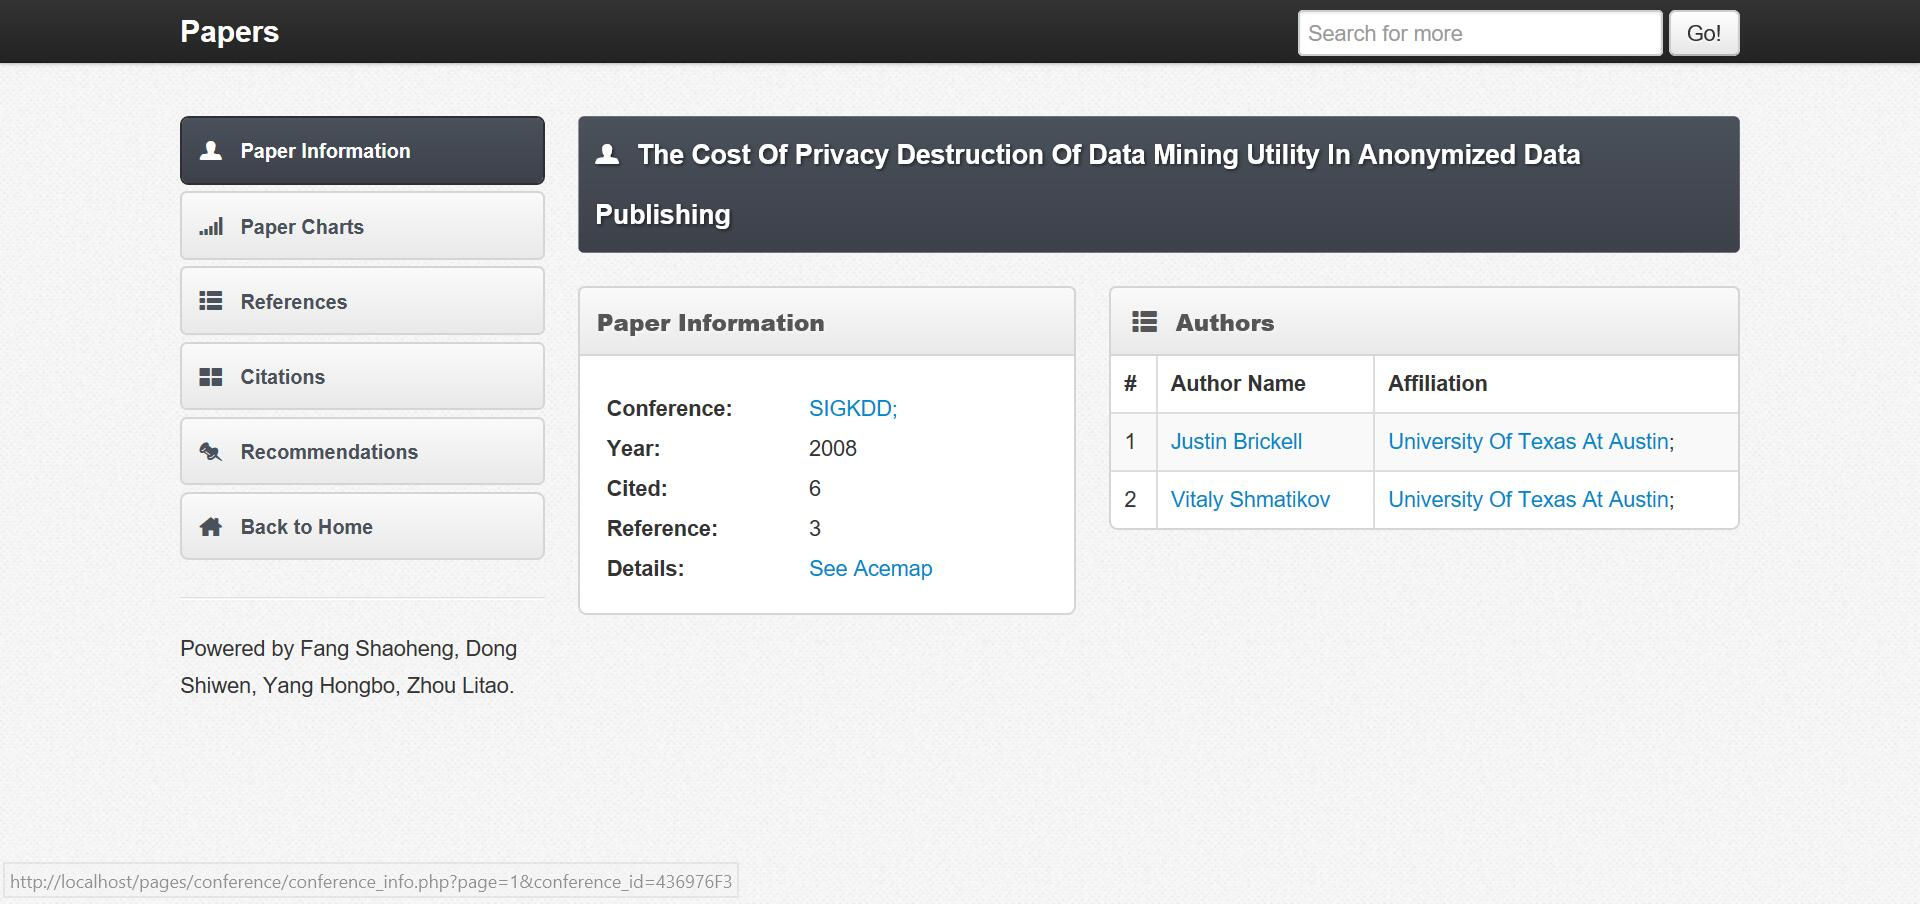
\includegraphics[height=7.0cm,width=16.0cm]{img/yhb_paper_1.jpg}
\caption{Page Example}
\end{figure}


Here we give code:
(Realization of Paper Charts will be introduced in chapter visualization.)
First, we have PaperID through ``Get'' method, then we can find result in MySQl. If result exists, we echo out all fields of paper-relavant  information. (Remember!  AuthorName is in the format of Arrays.)
\begin{figure}[H]
\centering
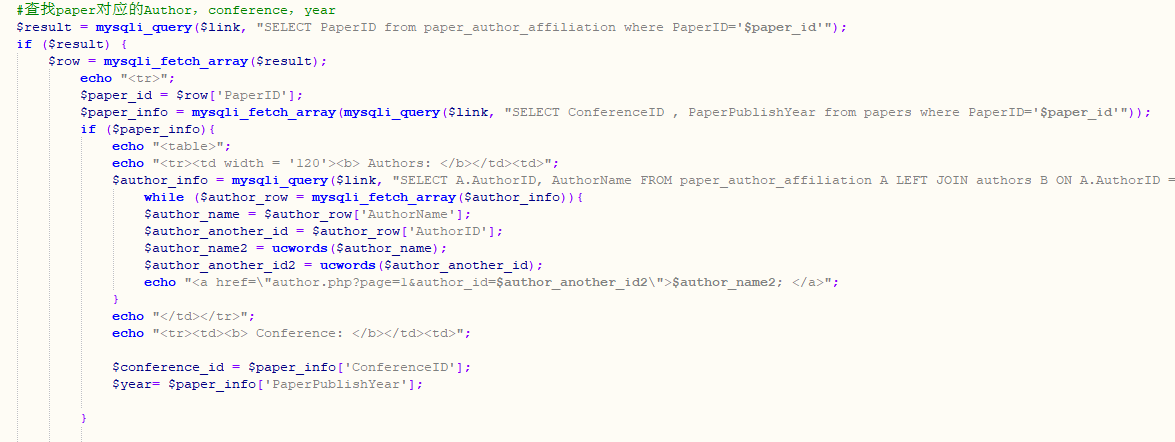
\includegraphics[height=8.0cm,width=16.0cm]{img/yhb_mp_1.png}
\caption{Code Example}
\end{figure}

\begin{figure}[H]
\centering
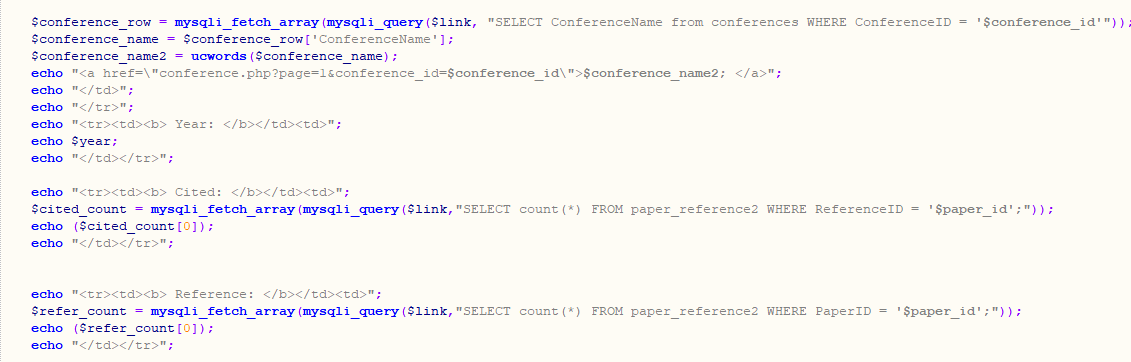
\includegraphics[height=8.0cm,width=17.0cm]{img/yhb_mp_2.png}
\caption{Code Example}
\end{figure}



\subsection{Paper: Citation and Reference}
This part is quite similar to paper information part(just add a loop if->while).
Before doing this, we should know what is thrown into MySQL. In the fuction above, that is PaperID, and in Reference part, it's ReferenceID while in Citation part, we swap paper and reference.

\begin{figure}[H]
\centering
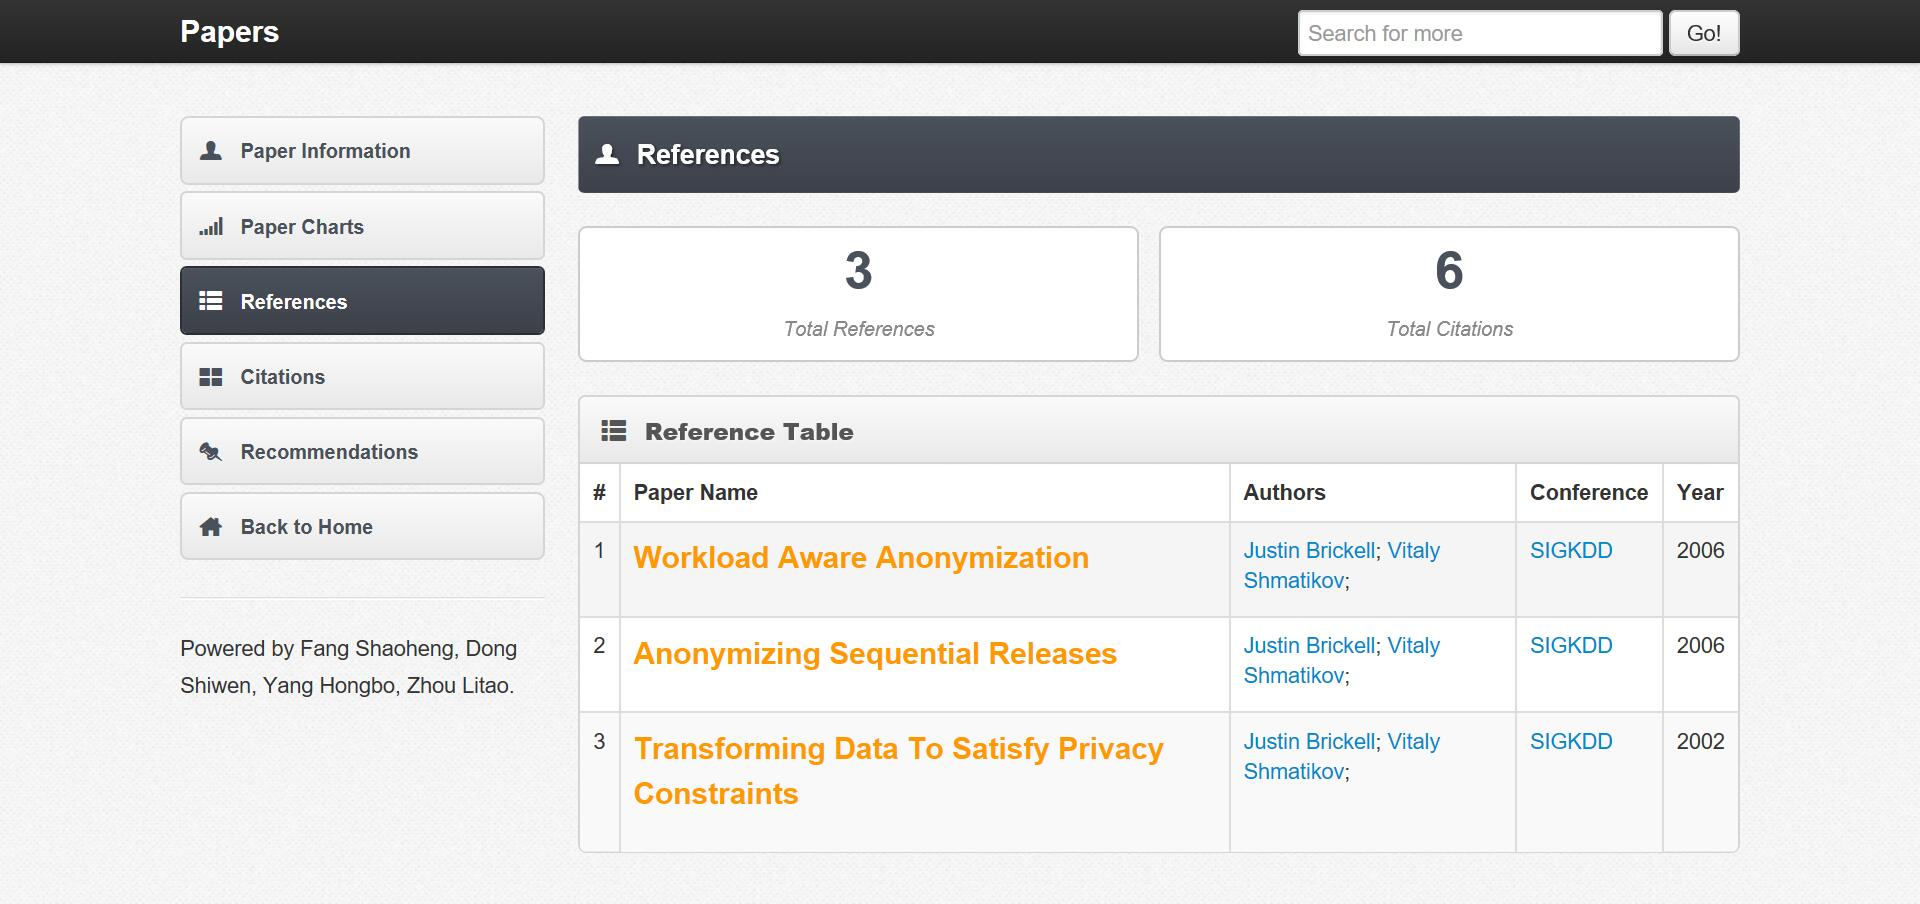
\includegraphics[height=6.0cm,width=16.0cm]{img/yhb_paper_2.jpg}
\caption{Page Example}
\end{figure}
Here we give code: (just the first part, the followed part has been already introduced.)
\begin{figure}[H]
\centering
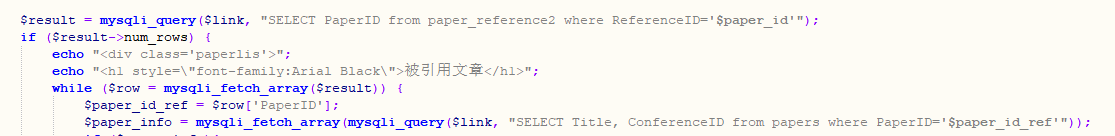
\includegraphics[height=3.5cm,width=16.0cm]{img/yhb_re_2.png}
\caption{Code Example}
\end{figure}

This is Citation Page example:
\begin{figure}[H]
\centering
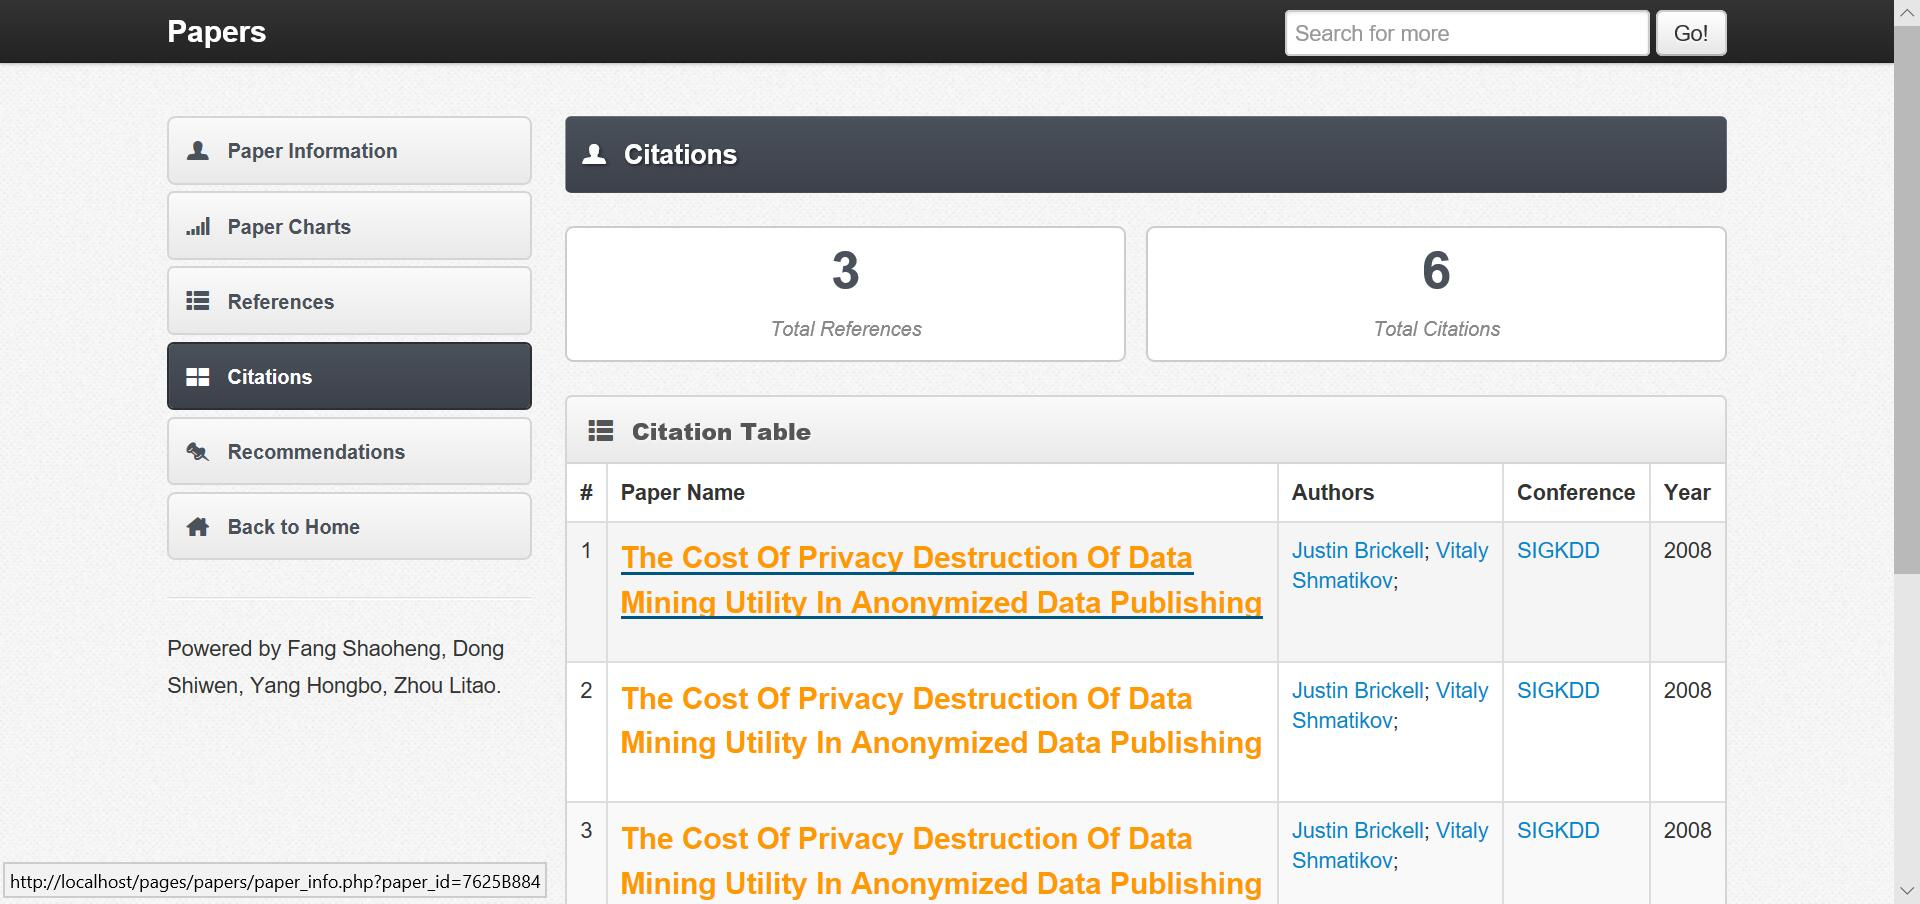
\includegraphics[height=7.0cm,width=16.0cm]{img/yhb_paper_3.jpg}
\caption{Page Example}
\end{figure}
Here we give code:
\begin{figure}[H]
\centering
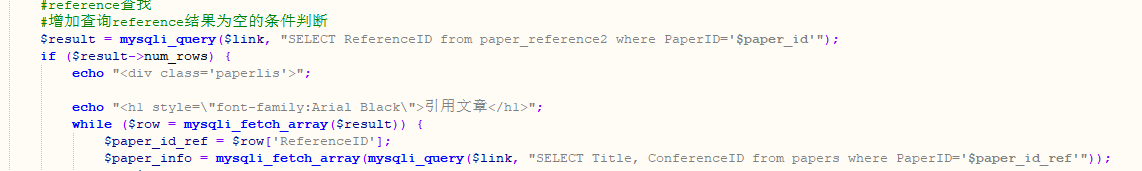
\includegraphics[height=3.5cm,width=16.0cm]{img/yhb_re_1.png}
\caption{Code Example}
\end{figure}




\begin{minipage}[r]{15em}
\begin{verbatim}


\end{verbatim}
\end{minipage}

\subsection{Paper: Recommand}
We came up with 2 method to recommend papers: 

\textbf{1) Recommend by relavant title}

This method relies on solr. In solr, field Title is stored as `text-en' format. So we can do vigrous search to match related papers First, we should search in MySQL to find Title (at the beginning, we have paper\_id ).
As the search result is in the format of (``    xxxxx   ''), 
we should process it to xxxxx to transmit to solr-url.
Specificly, we use   (var:)paper\_title4=substr((var:)paper\_title3,3,-2);


\begin{figure}[H]
\centering
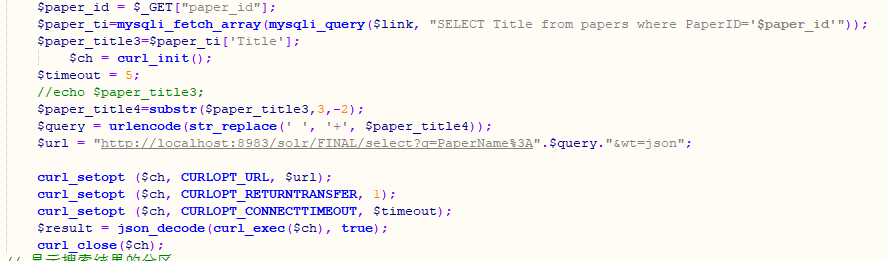
\includegraphics[height=6.0cm,width=16.0cm]{img/yhb_re_11.png}
\caption{Code Example}
\end{figure}

Then similarly, we can echo result out.
\begin{figure}[H]
\centering
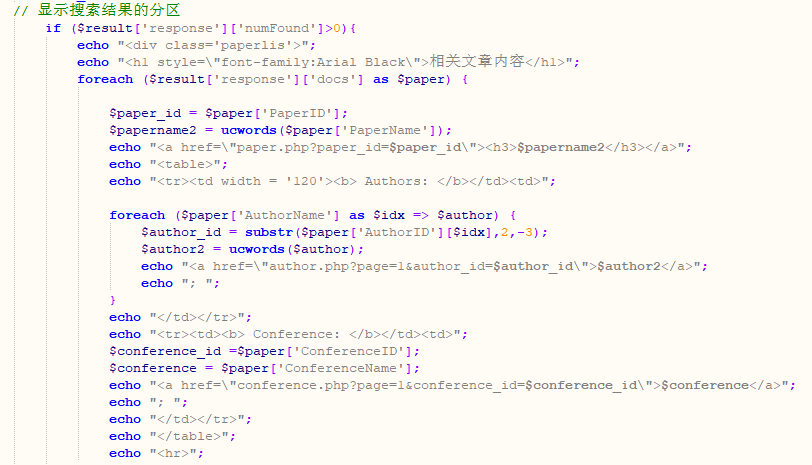
\includegraphics[height=10.0cm,width=18.0cm]{img/yhb_re_12.png}
\caption{Code Example}
\end{figure}

\textbf{2) Recommend by relavant Author}

This method relies on MySQL. The central sentence of this part is the MySQL join-query sentence below:
\begin{figure}[H]
\centering
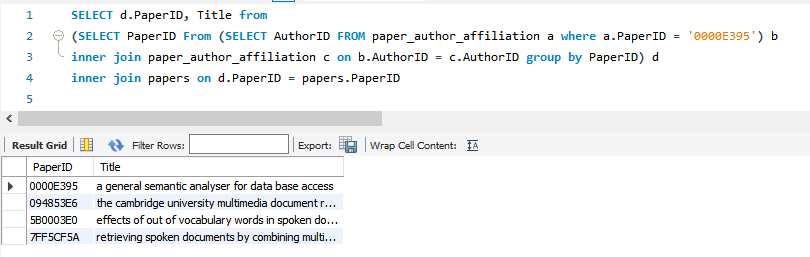
\includegraphics[height=4.0cm,width=13.0cm]{img/yhb_mp_4.png}
\caption{Code Example}
\end{figure}



Here we give complete codes:
\begin{figure}[H]
\centering
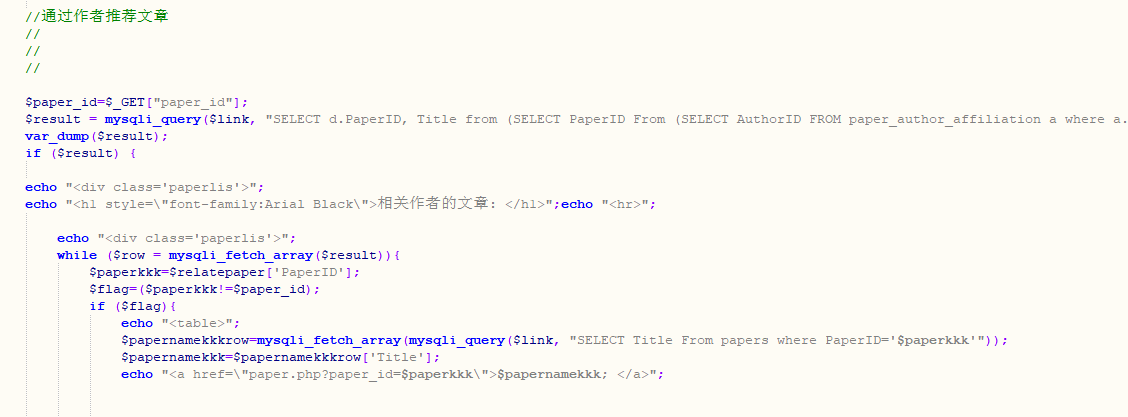
\includegraphics[height=7.0cm,width=16.0cm]{img/yhb_mp_3.png}
\caption{Code Example}
\end{figure}


Here we give exammple page:
\begin{figure}[H]
\centering
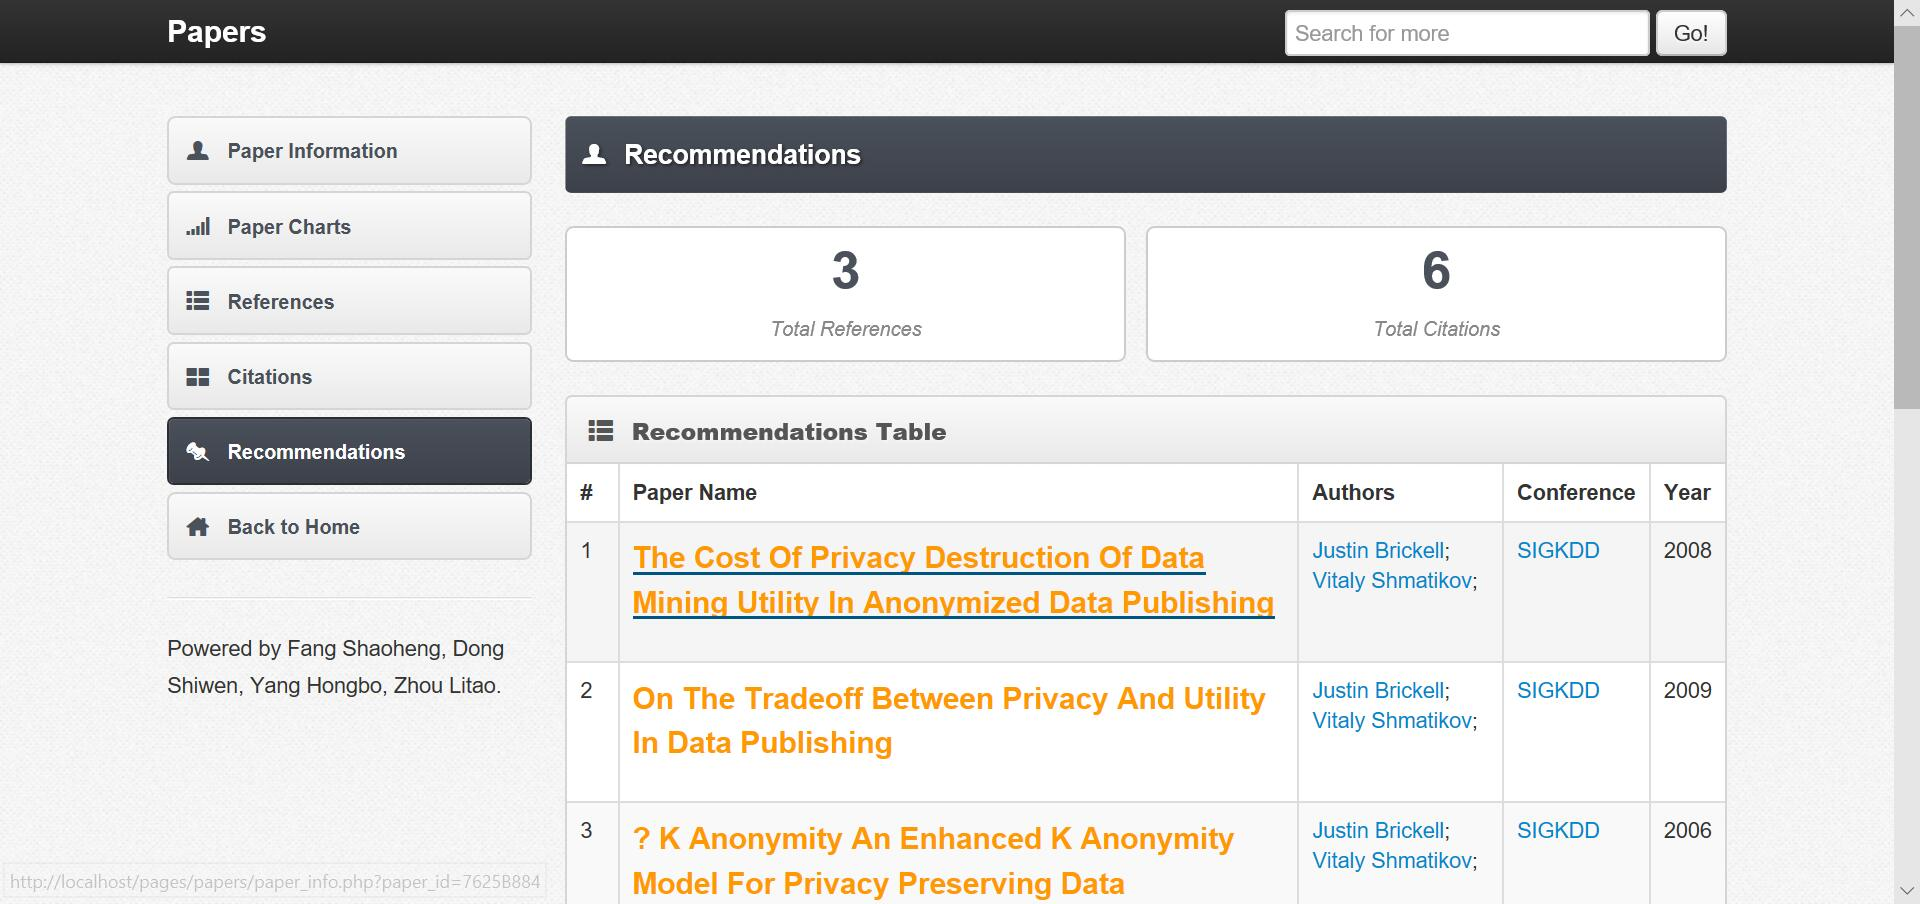
\includegraphics[height=7.0cm,width=16.0cm]{img/yhb_paper_4.jpg}
\caption{Page Example}
\end{figure}



\subsection{Conference Information}

In conference page, we showed basic information of conferences nameiy the number of authors, papers and references. Then we listed the papers that are included in the distinct conference and gave hyperlinks to other pages.

(The impletment of count function is shown in the next subsection.)
\begin{figure}[H]
\centering
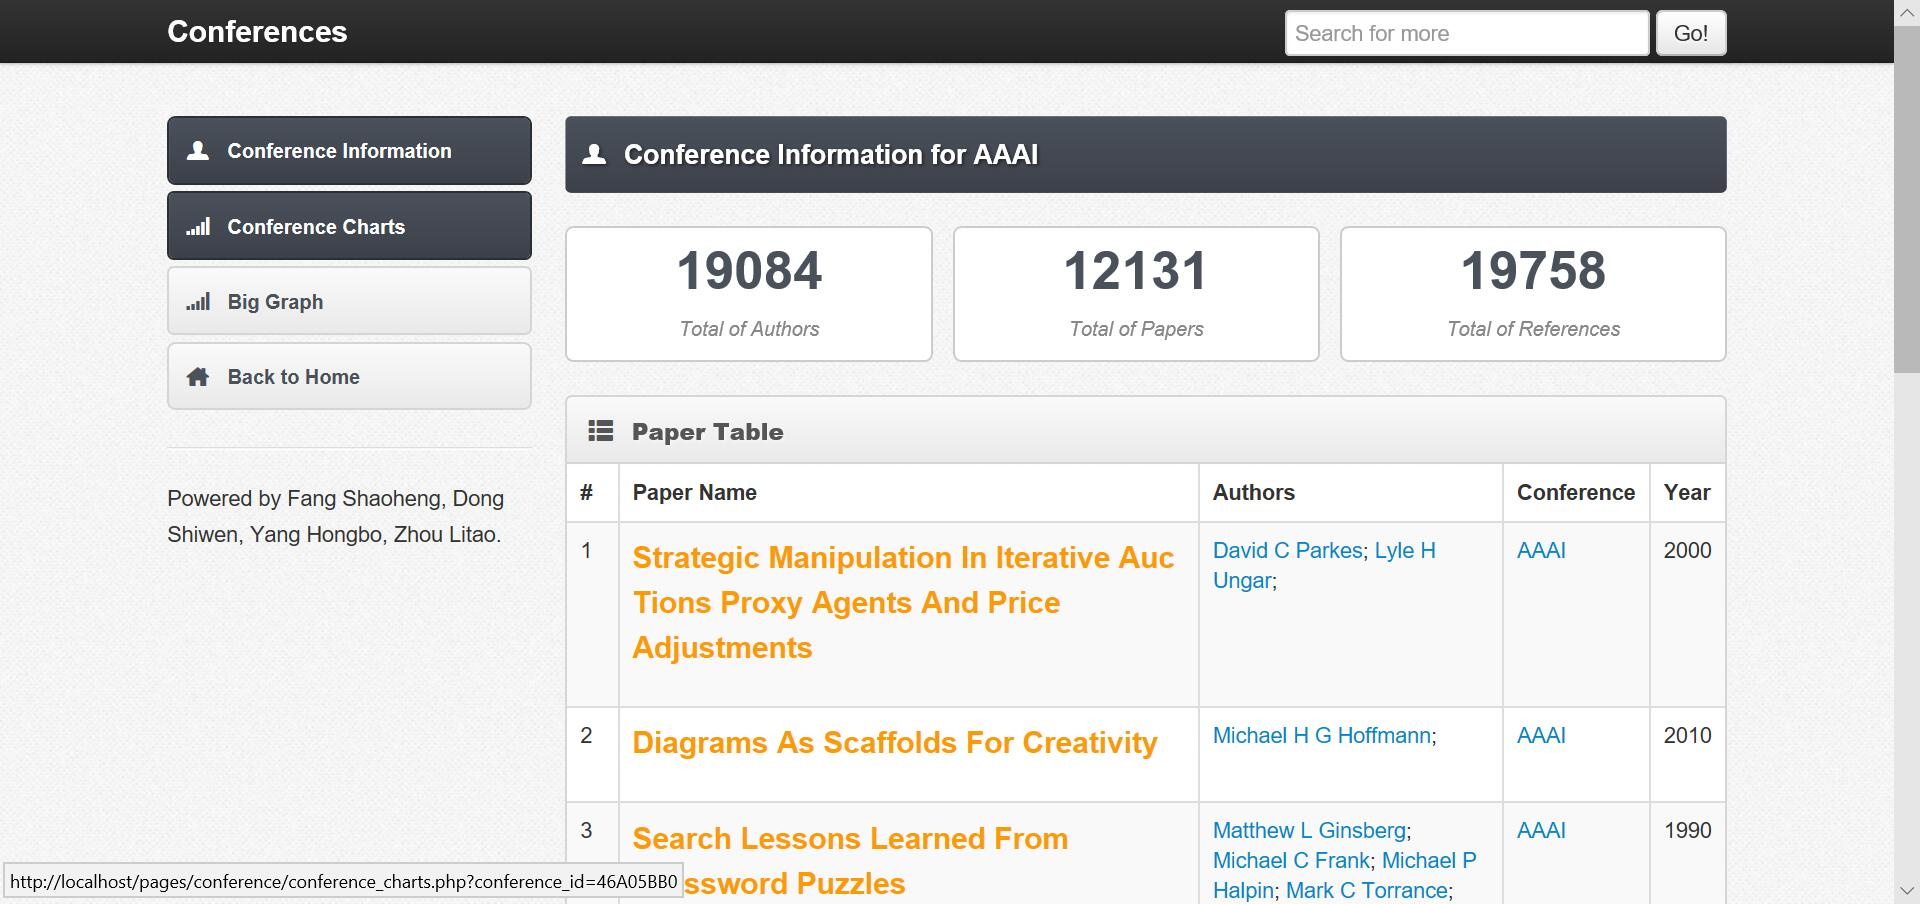
\includegraphics[height=7.0cm,width=16.0cm]{img/yhb_con_2.jpg}
\caption{Page Example}
\end{figure}
There are 3 blanks on the right side, which show the total number of authors, papers and references. We call this ``count function''. We wrote 2 versions. The first version use counting varaible in loops to count number, which is not  so efficient. So we turned to another method, which will be introduced in detail in ``affiliation page''.

Below these is a paper list.
Here is the code to search for papers that are included in the conference, the process to achieve  it is similar to that of ``author.php'' in last homework. We used MySQL to find the information we want. 

First, we have ConferenceID through `Get', then we can use code:
\begin{figure}[H]
\centering
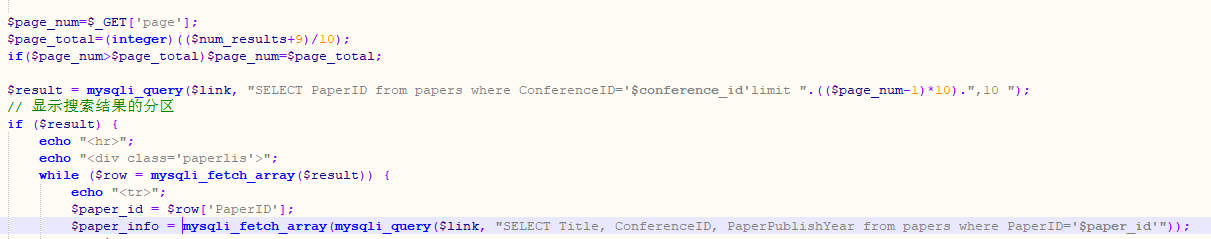
\includegraphics[height=4.0cm,width=16.0cm]{img/yhb_con_11.png}
\caption{Code Example}
\end{figure}


to find PaperID. And problem comes to using PaperID to find paper information.  We just follow the approach that was used in last homework, and echo the needed messages out. There is a point that should be mentioned. AuthorID field has multiple value, so we have to process like an array.
\begin{figure}[H]
\centering
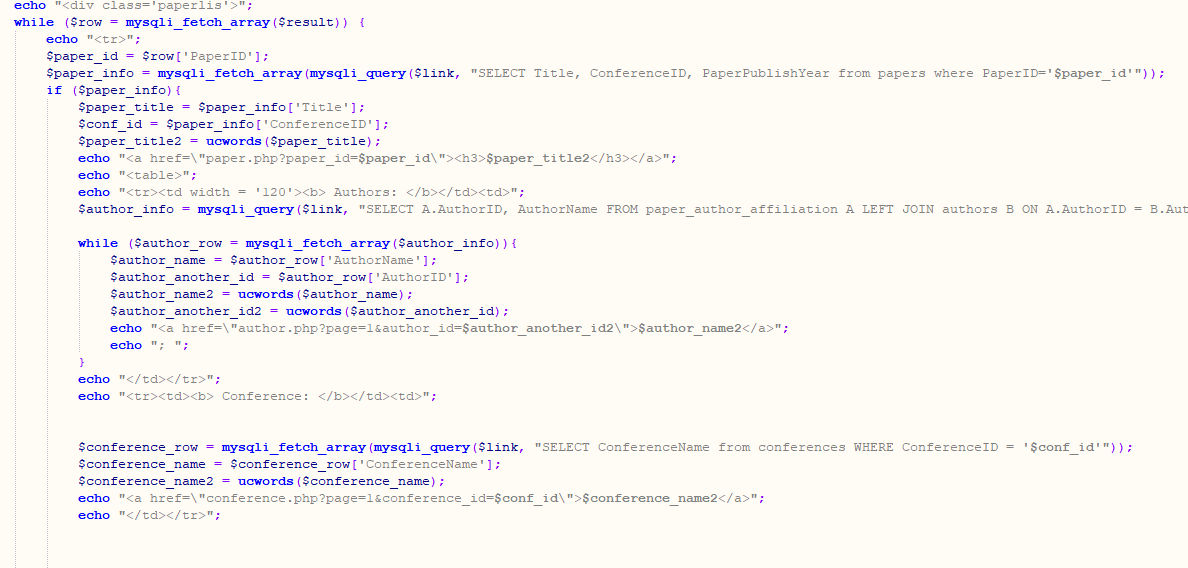
\includegraphics[height=8.0cm,width=16.0cm]{img/yhb_con_1.png}
\caption{Code Example}
\end{figure}


We also added E-charts and Gephi graphs in related pages to show the information of conference more clearly, which method will be discribed in detail in following chapters.



\section {Affiliation Pages}

We'd like to add a new series of pages to show affiliation information to users. Since we didn't do any previous work about affiliation information in the previous labs except that the affiliation table was input into the database, we have to write new SQL commands in search of affiliation information, and echo them out on the pages. The paper table and charts on other pages can be of help in showing the affiliation related information. Also, we have already got the author table written in the paper information page. Generally speaking, the work here is to collect the affiliation data and arrange them in order on the pages.


\subsection {General Description}

The final version of the affiliation section include 3 concrete pages. On the affiliation\_info.php page, we will give three numbers on top of the page, counting all the authors, papers, and references in the affiliation. Then the authors in the affiliation will be listed below, together with their own affiliation information (hyper-links included) and number of publications. Affiliation\_paper.php shows all the papers related to the affiliation. The affiliation\_charts.php, where three charts are displayed, will be reported in detail in the Statistical Graph Section.

\begin{figure}[H]
\centering
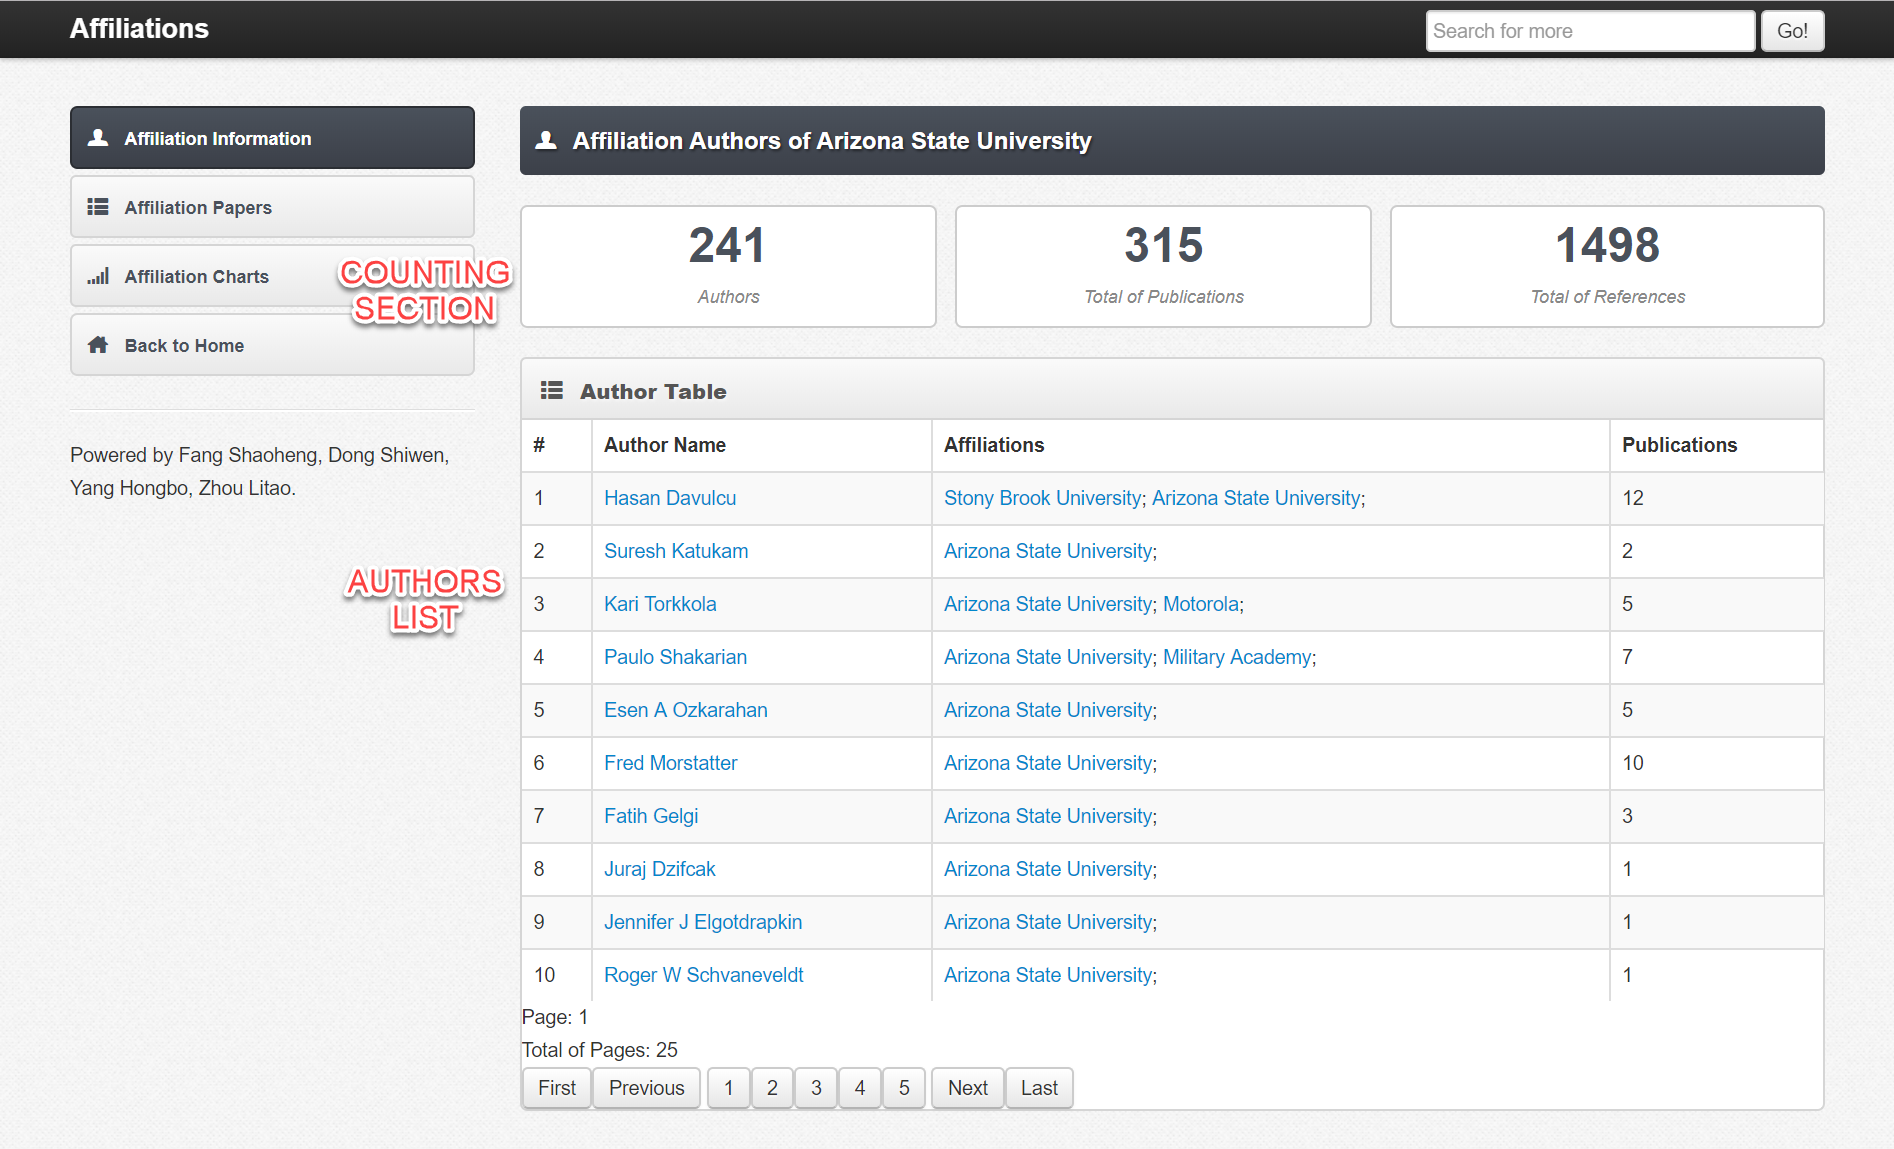
\includegraphics[scale=0.35]{img/zlt_aff_demo1.png}
\caption{affiliation\_info.php page}
\end{figure}

\begin{figure}[H]
\centering
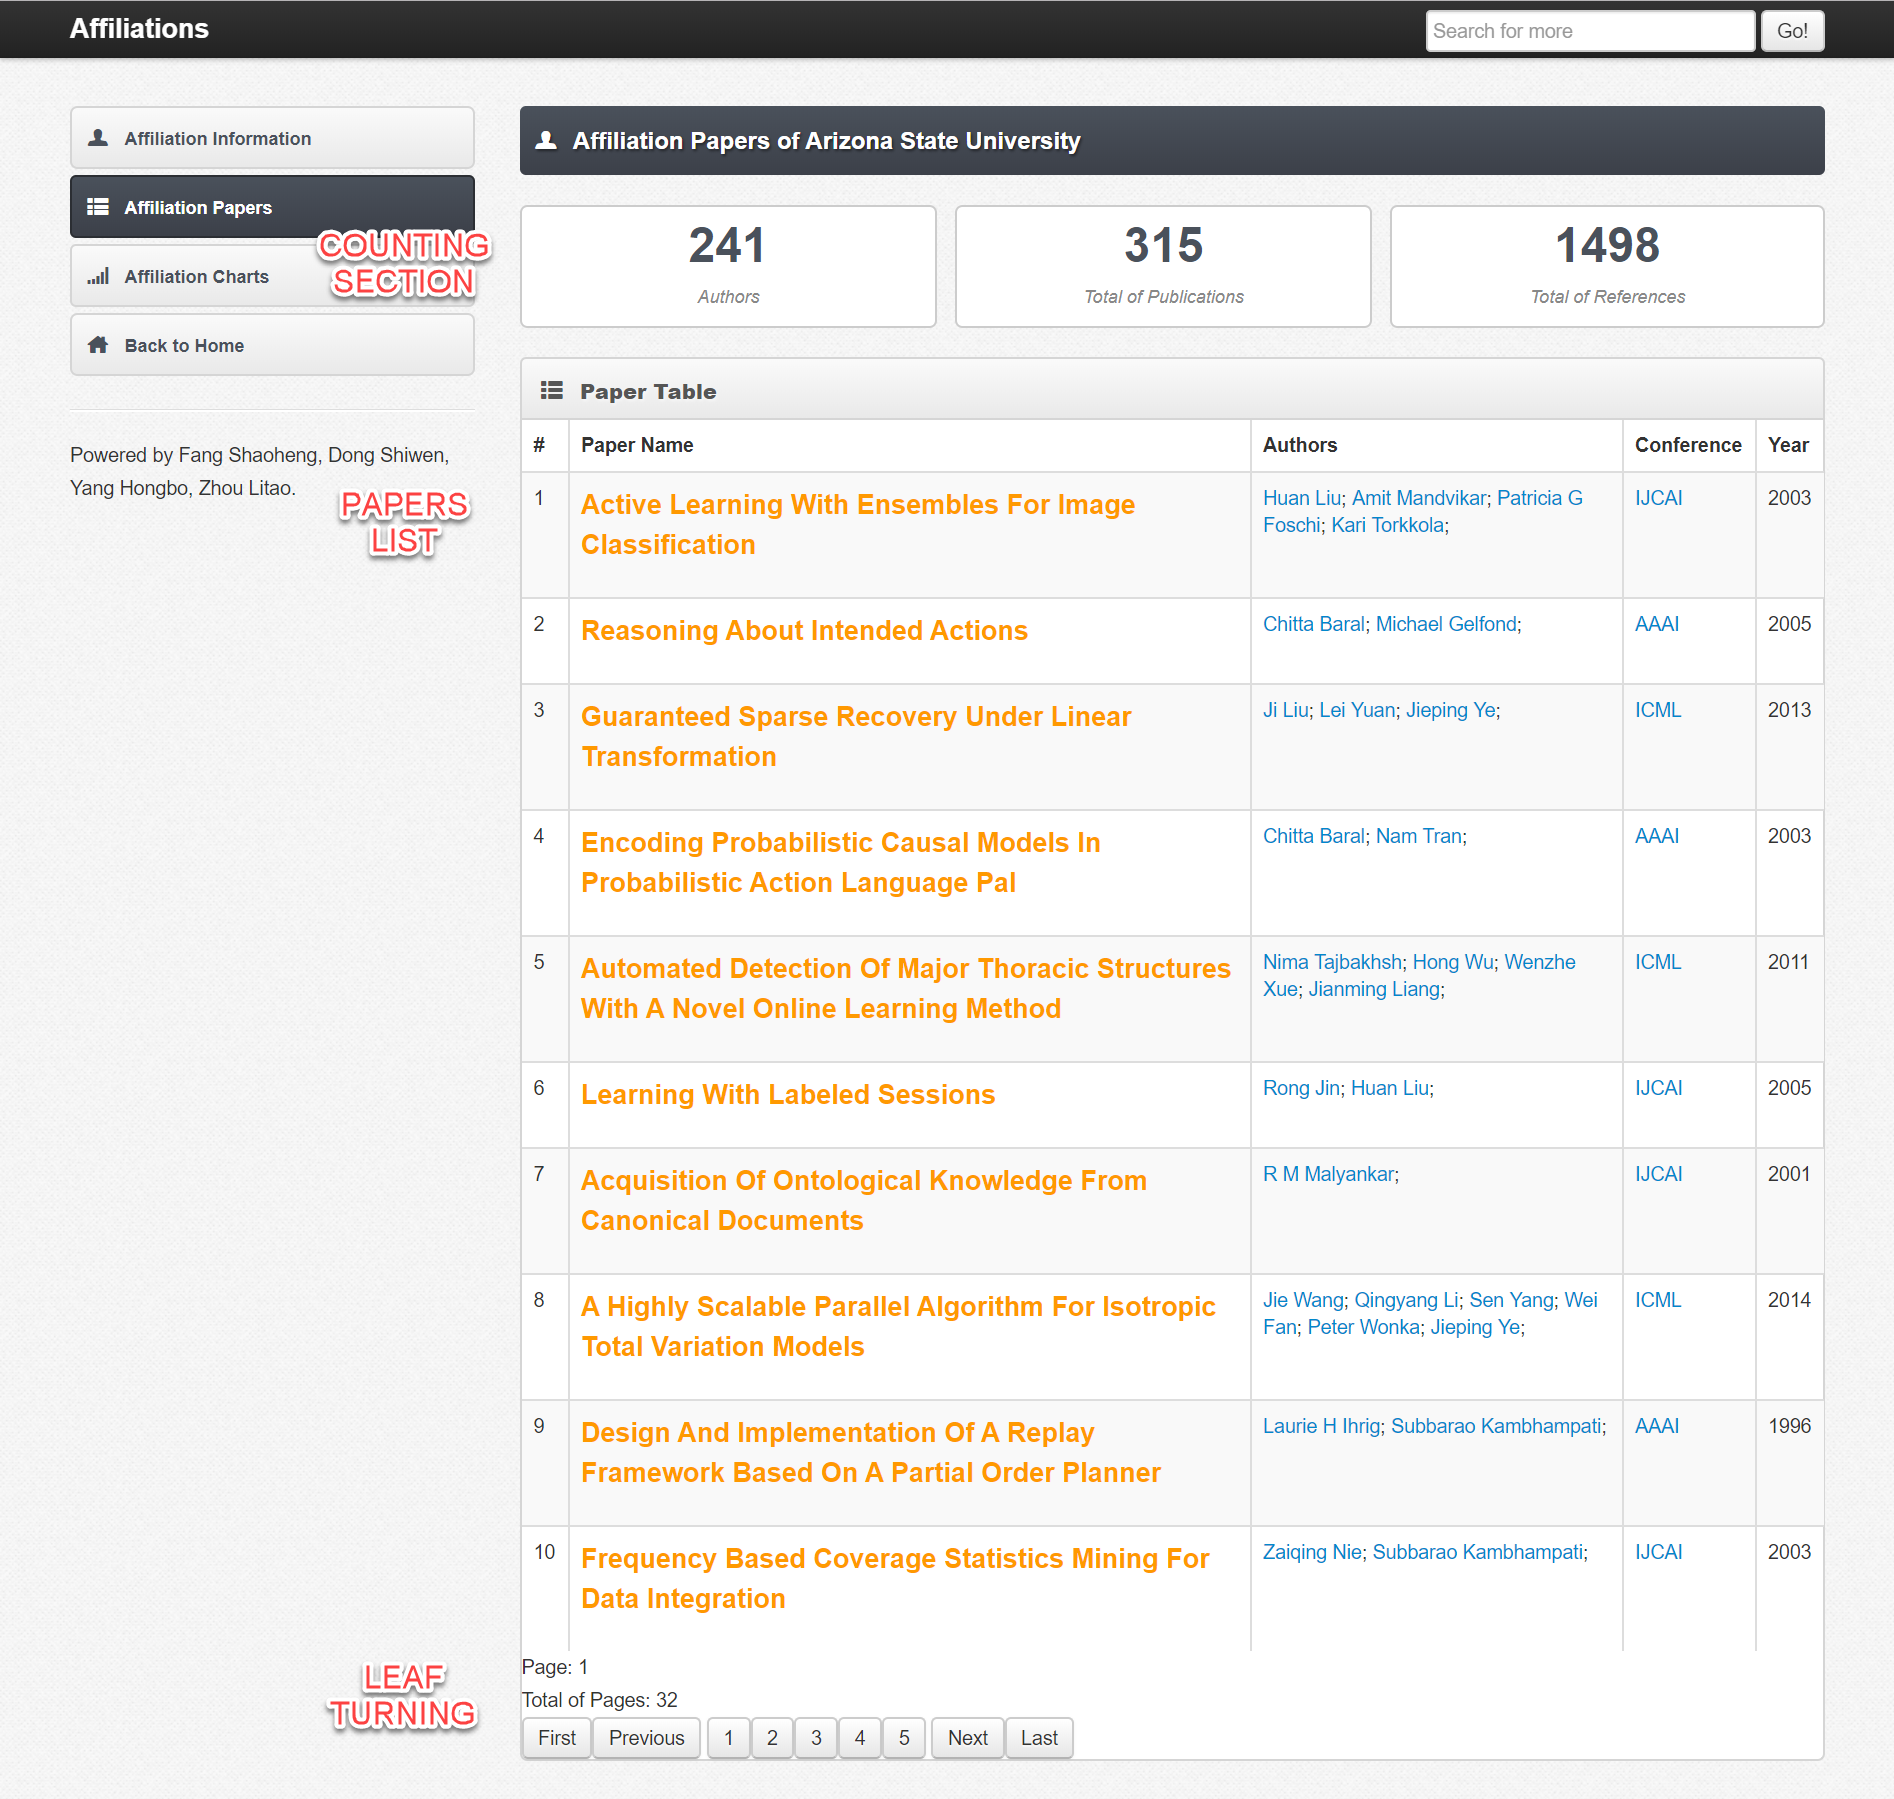
\includegraphics[scale=0.35]{img/zlt_aff_demo2.png}
\caption{affiliation\_paper.php page}
\end{figure}

In fact, for the same function to be displayed on the page, we did two versions of code to implement them. The first one was very basic, just like those in the paper/author/search pages. However, since all the affiliation data are selected from the big paper\_author\_affiliation table, the first version didn't perform well in loading speed. Our optimization will be introduced in the Optimization Chapter.



\subsection {Total Counts}
On top of every affiliation page, we've counted all the authors, papers and references concerned. For authors and papers, we can directly count them in the paper\_author\_affiliation table. For references, we first select the papers and then join the selected results to the paper\_reference table in order to count the results. The MySQL commands are listed below.

\begin{figure}[H]
\centering
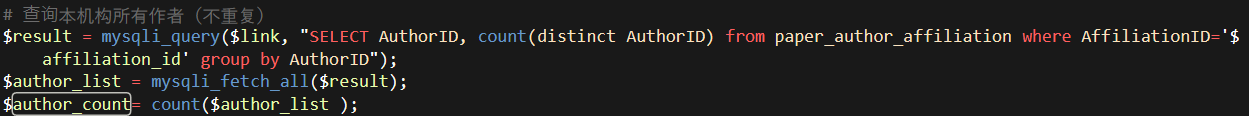
\includegraphics[scale=0.55]{img/zlt_aff_authorcount.png}
\caption{Count Author Commands}
\label{fig:aff_authorcount}
\end{figure}
\begin{figure}[H]
\centering
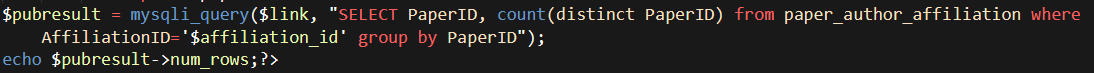
\includegraphics[scale=0.6]{img/zlt_aff_papercount.png}
\caption{Count Paper Commands}
\label{fig:aff_papercount}
\end{figure}
\begin{figure}[H]
\centering
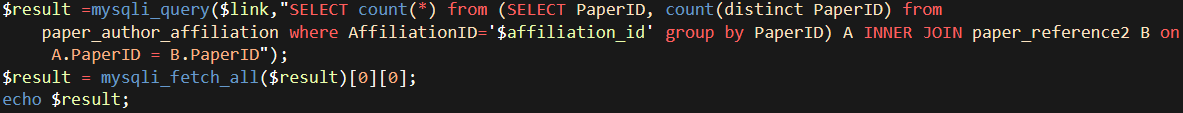
\includegraphics[scale=0.55]{img/zlt_aff_refcount.png}
\caption{Count Reference Commands}
\label{fig:aff_refcount}
\end{figure}

Note that we've use some MySQL techniques such as DISTINCT (eliminate overlapping results) and GROUP BY (perform data counting job) in order to implement our function.

For the data display in our page, our template has already provided a well designed data container in CSS, which can list different numbers in a row, with even width. We can simply apply this pre-defined class in a way demonstrated below.

\begin{figure}[H]
\centering
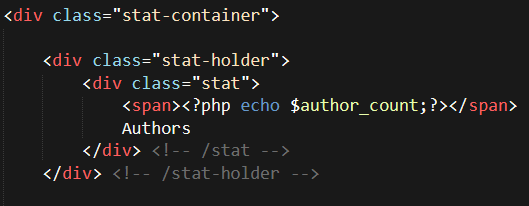
\includegraphics[scale=0.8]{img/zlt_aff_countdisplay.png}
\caption{Use Pre-defined Class to Display Numbers}
\end{figure}


\subsection{Authors List}

The author we've found based on the given affiliaiton may have more than one affiliation where he publishes his paper. So one simple search work is not enough. Luckily, all of the data related to this problem can be selected from the paper\_author\_affiliation table. As a result, our first design is to first sort out all the authors where the affiliation column fits, then we search the table again for affiliation information based on the author's id, which can be realized by looping through the author array in PHP.

In fact, the first step has been done when we count the authors (See Figure \ref{fig:aff_authorcount}), so we simply skip the first step, call the author selecting result in the counting section, and make further searching based on the previous result. During the second step, we've also used DISTINCT \& GROUP BY techniques in order to get the author's affiliation data right and unrepeated.

\begin{figure}[H]
\centering
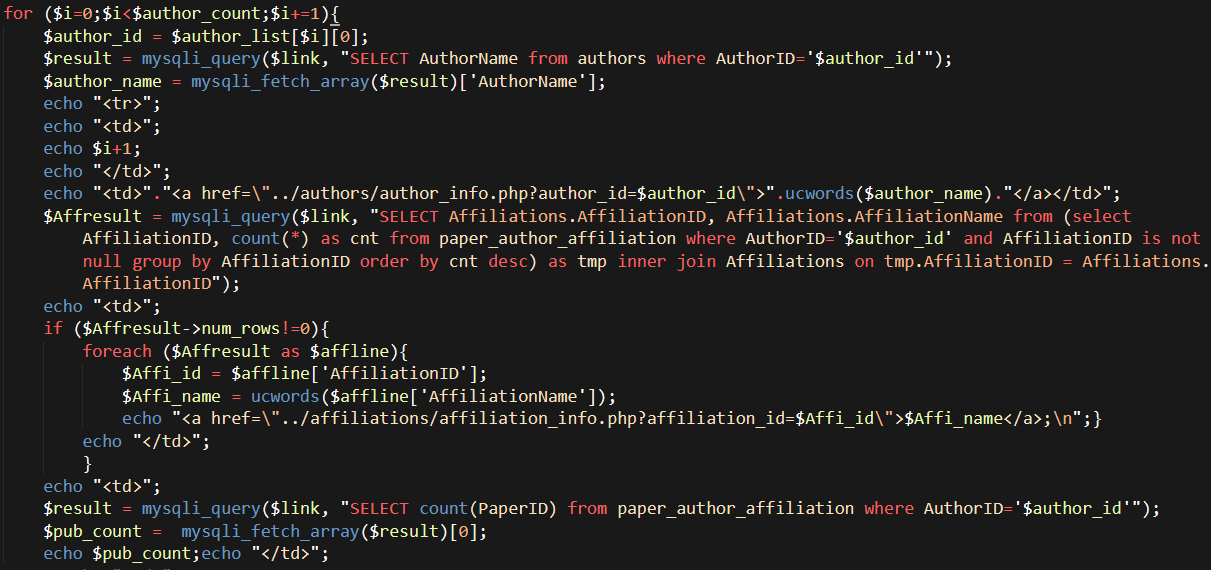
\includegraphics[scale=0.55]{img/zlt_aff_authorloop.png}
\caption{Use Loop to List Author\_Affiliation Information}
\end{figure}

The problem with this solution is that the searching work is too much. Imagine there are 100 authors related to one affiliation, we have to go through the big paper\_author\_affiliation table 100 times in order to get all the data. It turned out that it would take the webpage about half a minute to get completed loaded. The optimization work will be introduced in the Optimization Chapter.

\subsection{Papers List}

The general structure of this list is simlilar to those in citation/ reference/ author's paper list. We may just use MySQL to select all the paper's id related to the affiliation, keep this array storing the paperid we want to display, and the leave the rest of the work to the codes we've already written in the previous work. The selecting MySQL commands are listed below. Actually, just like the case in the author list section, the first step has also been completed in the counting section. (See Figure \ref{fig:aff_papercount}) So there are no codes left for this section to explain.

\chapter{Leaf Turning}

dsw

\section{Version I: by PHP parameters}

\subsection{Description}

\subsection{Solution}

\paragraph{point 1}

\paragraph{point 2}

\subsection{Source Codes}

\begin{minipage}[r]{15em}
\begin{verbatim}

short code example

\end{verbatim}
\end{minipage}

\subsection{Explanation}

\subsection{Demonstration}

\begin{figure}[H]
\centering

\includegraphics[height=4.0cm,width=4.0cm]{img/dsw_1.jpg}
\caption{IMG EXAMPLE}
\end{figure}


\section{Version II: by jQuery}



\chapter {Integrated Searching Bar}

fsh


\chapter {Data Visualization}


\section {Statistical Graph}

fsh

\subsection{Description}

\subsection{Solution}

\paragraph{point 1}

\paragraph{point 2}

\subsection{Source Codes}

\begin{minipage}[r]{15em}
\begin{verbatim}

short code example

\end{verbatim}
\end{minipage}

\subsection{Explanation}

\subsection{Demonstration}

\begin{figure}[H]
\centering

\includegraphics[height=4.0cm,width=4.0cm]{img/fsh_1.jpg}
\caption{IMG EXAMPLE}
\end{figure}



\section {Paper Relation Graph}

zlt

\subsection{Description}

\subsection{Solution}

\paragraph{point 1}

\paragraph{point 2}

\subsection{Source Codes}

\begin{minipage}[r]{15em}
\begin{verbatim}

short code example

\end{verbatim}
\end{minipage}

\subsection{Explanation}

\subsection{Demonstration}


\section{Big Charts using Gephi}

As the saying goes, ``One picture worths 1000 words.'', a visualization picture is vital to show the connection between objects in some scales. To show an overall relationship, we choose  \textbf{gephi} to visualize the data collected by MySQL. This method can help the part of E-charts to draw a better pictue in users' mind. 
There was a problem that troubled us for a long time. That is: how can we put the picture onto the pages. And it is finally solved by using package ``ariutta/svg-pan-zoom
'' from GitHub. 
Here we'll give MySQL sequences and the way to draw a gephi picture(.svg).

\subsection{MySQL Fetch}

We choose to show the connection between authors in all 13 conferences. We established the connection by reference and citation. And this demands us to use `join search' in MySQL. Example codes are given below.(We take ConferenceID= `47c39427' for an example.)

\begin{figure}[H]
\centering

\includegraphics[height=4.0cm,width=18cm]{img/yhb_my_1.png}
\caption{search example}
\end{figure}

Finally, remember to lead the data out in (.csv) format, in order that we can use the data in gephi easily.

\subsection{Gephi Drawing}

Gephi can use data in (.csv) format directly. After transmitting information into gephi, we can find a picture in the window. But this picture is so ugly and unclear that we cannot take it for visualization use derectly.  

\begin{figure}[H]
\centering

\includegraphics[height=7.0cm,width=18.0cm]{img/yhb_ge_1.png}
\caption{geghi: original picture}
\end{figure}
We may turn to gragh-drawing methods such as ``force directed method'' and ``Fruchterman Reingold method'', to better display the characteristics of the relationship between authors.

Next, we can adjust the  size of each node by degree, and give them different colors.
It's much easier for us to see the relation.
\begin{figure}[H]
\centering
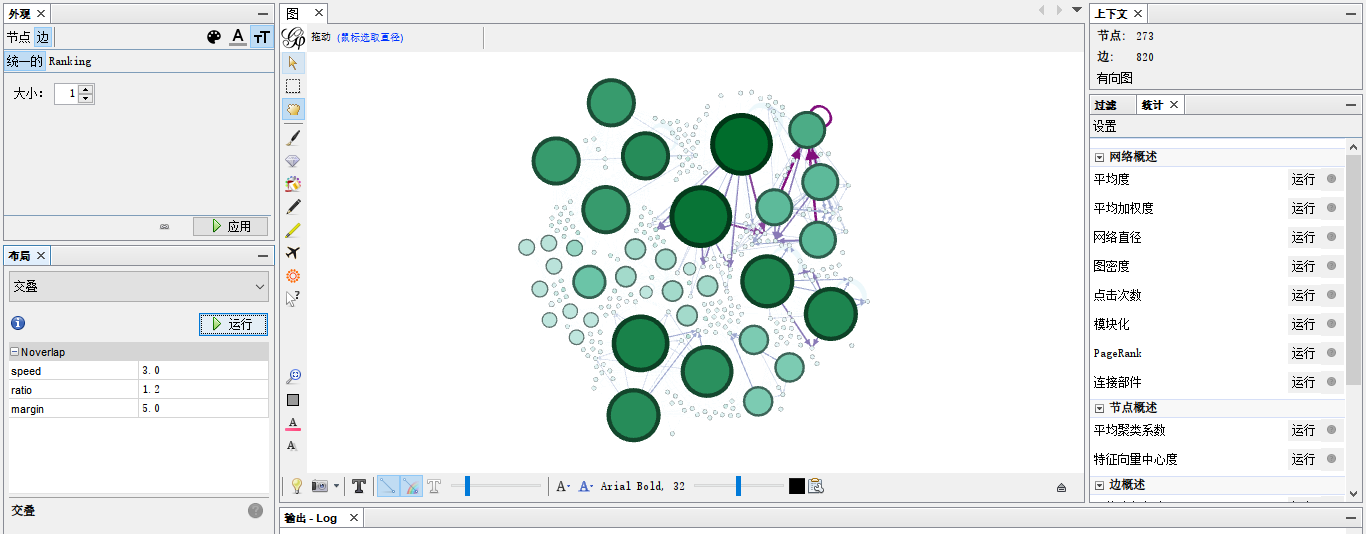
\includegraphics[height=7.0cm,width=18.0cm]{img/yhb_ge_2.png}
\caption{geghi: processed picture}
\end{figure}
Finally, we can transmit it as (.svg) file to load on the pages.

\chapter {Beautify the Pages}

\section {Index Beautification}

fsh

\section {Information Pages Beautification}

zlt


\chapter {MySQL Optimization in Affiliation Pages}

zlt

\end{document}
